%%%%%%%%%%%%%%%%%%%%%%%%%%%%%%%%%%%%
%%% Modelo de documento LATEX    %%%
%%% autor: Leandro do Nascimento %%%       
%%% Data: 25/julho/2020           %%%
%%%%%%%%%%%%%%%%%%%%%%%%%%%%%%%%%%%%

%% Classes de documento, frente e verso, tamanho da fonte, papel
\documentclass[12pt,a4paper,oneside]{article}

%% Define margens, superior, inferior, direta e esquerda
\usepackage[a4paper,top=3cm,bottom=2cm,left=3cm,right=2cm]{geometry}

\usepackage[utf8]{inputenc}   %%% Acentuar palavras
\usepackage[brazil]{babel}    %%% Define idioma do documento 
\usepackage{graphicx}         %%% Permite inserir figuras
\usepackage{float}            %%% Permite configurar figuras
\usepackage{trivfloat}        %%% Permite inserir novos tipos "float"
\usepackage{setspace}         %%% Permite configurar distancia entre linhas
\usepackage{hyperref}         %%% Permite utilizar links no texto
\usepackage{colortbl}         %%% Usar biblioteca de cores
%\usepackage{indentfirst}	  %%% Indenta 1º parágrafo de cada seção.
\usepackage[alf]{abntex2cite} %%% Estilo das Referências Bibliográficas
\usepackage{fancyhdr}  %utiliza biblioteca de cabeçalho e rodapé
\usepackage{pdfpages}         %%% Permite inserir arquivos PDF no texto
%\usepackage{times}                         %%% Troca para fonte TIMES
%\usepackage{helvet}                        %%% Troca para fonte HELVET
%\renewcommand{\familydefault}{\sfdefault}  %%% Troca para fonte HELVET

\setlength{\parindent}{1.5cm} %%% Distancia da primeira linha à margem
\setlength{\parskip}{9pt}     %%% Distancia entre parágrafos
\setstretch{1.0}              %%% Distância entre linhas

\trivfloat{quadro}            %%% Da novo à um novo float
\floatstyle{plaintop}         %%% Define a posição título do novo float

\definecolor{corleandro1}{RGB}{102,51,0}   %%% Nomeia uma nova cor
\definecolor{corleandro2}{RGB}{128,0,128}  %%% Nomeia uma nova cor

%#################################################################%
%## INÍCIO DO DOCUMENTO ##########################################%
%#################################################################%
\begin{document} 

%%LDN Configurações do CABEÇALHO e RODAPÉ
\pagestyle{fancy} % permite alterar cabeçalho e rodapé
\renewcommand{\headrulewidth}{0.5pt}
%\renewcommand{\footrulewidth}{0.5pt}
\lhead[\thepage]{} % esquerda do cabeçalho
\chead{} % centro do cabeçalho
\rhead[]{\thepage} % direita do cabeçalho
\lfoot{} % esquerda do rodapé
\cfoot{} % centro do rodapé
\rfoot{} % direita do rodapé

%%% Início CAPA DO DOCUMENTO %%%%%%%%%%%%%%%%%%%%%%%%%%%%%%%%%%%%%%
\begin{titlepage}
\centering
\textsc{\large FACULDADE DE TECNOLOGIA DE SÃO PAULO - FATEC}\\[0.2cm]
\textsc{\large FATEC SÃO CARLOS}\\[0.2cm]
\textsc{\large GESTÃO EM RECURSOS HUMANOS}\\[0.2cm]
%%% Início FIGURA DA CAPA %%%%%%%%%%%%%%%%%%%
\begin{figure} [H] 
\centering

\includegraphics[scale=0.35]{Fig/Logo Fatec.jpg} 
\end{figure}
%%% Fim da FIGURA %%%%%%%%%%%%%%%%%%%%%%%%%%%
\vfill
{ \LARGE \bf Comportamento Organizacional - Análise do documentário Indústria Americana (2019) }
\vfill
{ \large \bf Prof. Marcio Alves Silveira }
\vfill
{ \large \bf Leandro do Nascimento}
\vfill
{\large São Carlos\\Julho de 2020 }
\end{titlepage}
\thispagestyle{empty} %%% Oculta o número da capa
%%% FIM CAPA DO DOCUMENTO %%%%%%%%%%%%%%%%%%%%%%%%%%%%%%%%%%%%%%%%%



%%% Início COSTAS DA CAPA %%%%%%%%%%%%%%%%%%%%%%%%%%%%%%%%%%%%%%%%%
\newpage
\thispagestyle{empty} %%% Oculta o número das costas da capa
%%% Fim COSTAS DA CAPA%%%%%%%%%%%%%%%%%%%%%%%%%%%%%%%%%%%%%%%%%%%%% 

%%% Início do Cabeçalho e Rodapé
%%%%%%%%%%%%%%%%%%%%%%%%%%%%%%%%%%
\cleardoublepage        %%% Inicia próxima página em uma ímpar
\tableofcontents        %%% insere o sumário


%%% Início DO TEXTO (Capitulo 1) %%%%%%%%%%%%%%%%%%%%%%%%%%%%%%%%%%
\cleardoublepage        %%% Inicia próxima página em uma ímpar
\setcounter{page}{1}    %%% Começa a numerar aqui na página 1


\begin{onehalfspace}

\section{Sobre a produção do documentário}

\textbf{Título:} American Factory (Indústria Americana)\\
\textbf{Ano:} 2019 \\
\textbf{Direção:} Steven Bognar e Julia Reichert \\
\textbf{Produção:} Jeff Reichert e Julie Parker Benello \\
\textbf{Prêmios:} Vencedor do Oscar 2020 na categoria de melhor documentário \\
\textbf{Observação:}  \textit{É o primeiro filme da produtora do casal Barack Obama e Michelle Obama, Higher Ground Productions.
}

%%% Estrutura para inserir uma FIGURA %%%%%%%%%%%%%%%%%%%%%%%%%%%%%
\begin{figure} [H]
\centering
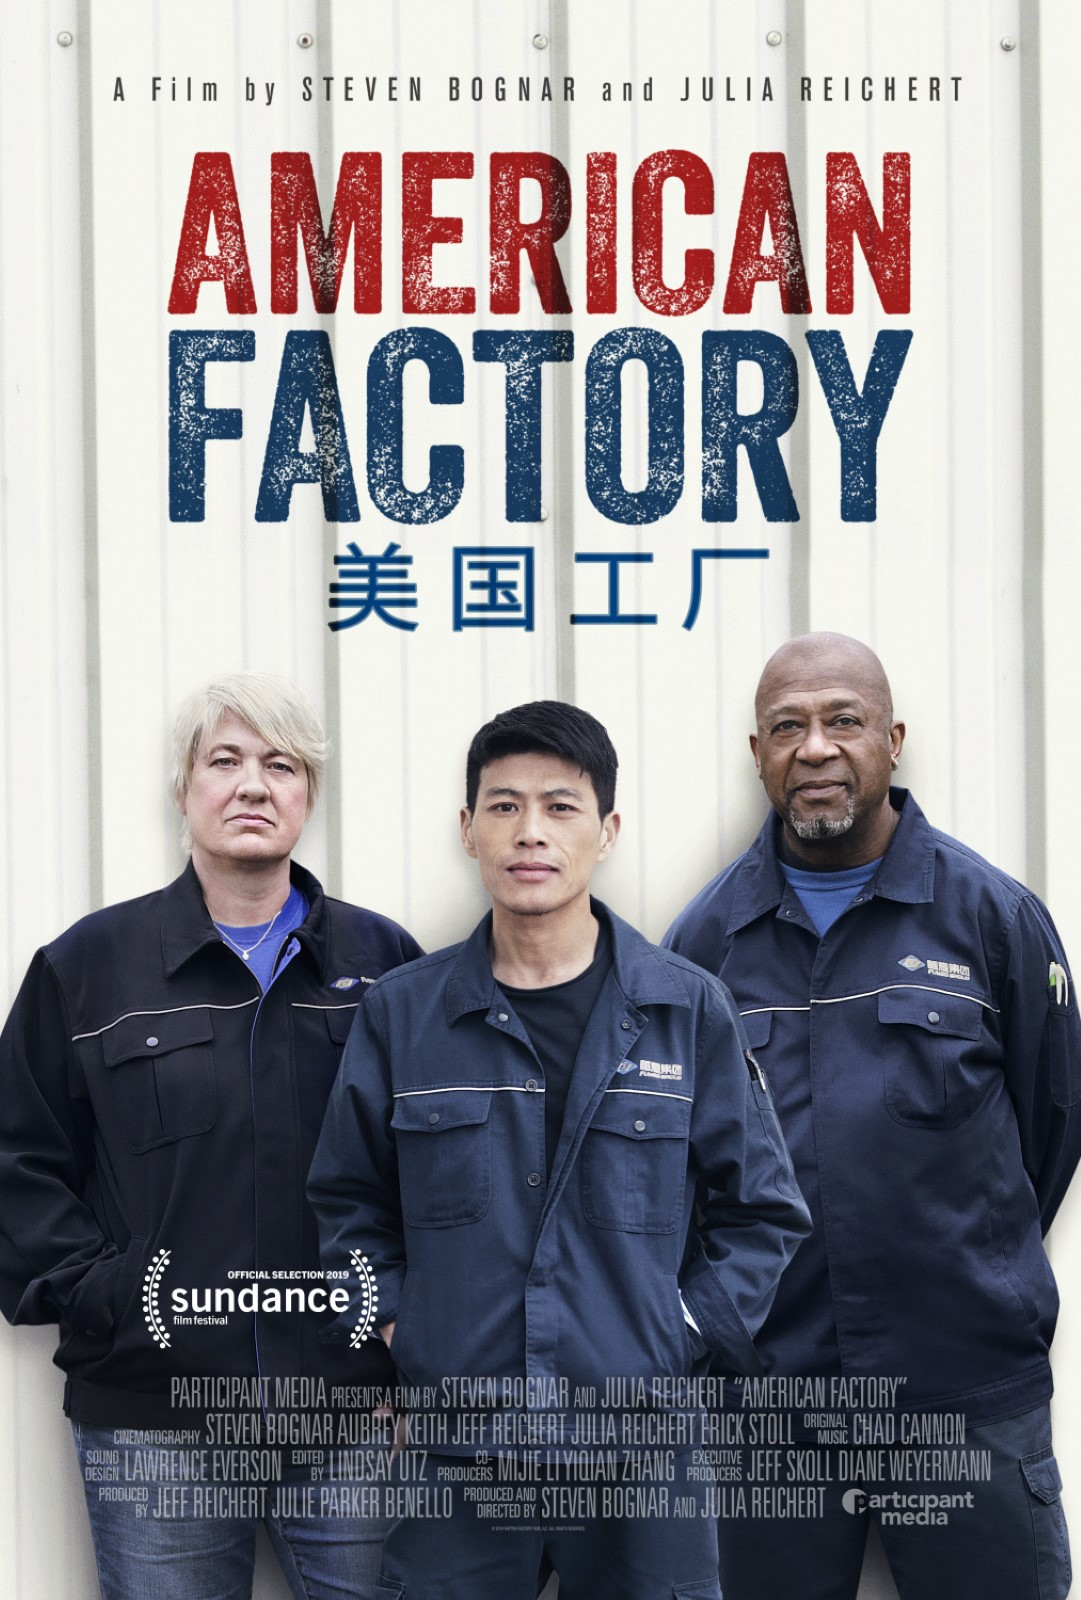
\includegraphics[scale=0.3]{Fig/AmericanFactory.jpg} 
\caption{Capa do documentário American Factory}
\label{fig:MapGrandNaveg}
\end{figure}
%%%%%%%%%%%%%%%%%%%%%%%%%%%%%%%%%%%%%%%%%%%%%%%%%%%%%%%%%%%%%%%%%%%

\newpage
\section{Análise do documentário Indústria Americana}

\hspace{1.5cm} Partindo do pressuposto de que a \textbf{Globalização} é entendida como o processo de expansão e integração da política, cultural e principalmente da economia entre os países, o documentário Indústria Americana é um claro exemplo prático disso.

O documentário retrata, de maneira eficiente, um processo prático de globalização. O longa mostra a inauguração da empresa chinesa, especializada na fabricação de vidros automotivos, a FUYAO. A China após a sua abertura econômica na década de 70, foi ganhando espaço no mercado e se tornou a segunda maior potência mundial. Ná época da compra a China estava em seu auge, o que foi possível um investimento chinês de alguns milhões do dólares para instalar-se no EUA.
A história que é contada de maneira linear inicia-se com a compra de um galpão, onde antes funcionava a empresa General Motors (GM), falida com a crise de 2008, no estado de Ohio nos Estados Unidos.

No ínicio, a instalação da empresa chinesa parece ser uma grande oportunidade para as pessoas que moram nas proximidades e que trabalhavam na GM, se sentem empolgadas com a inauguração. A empresa é trazida como um ótimo negócio chinês e que por meio da parceria com os Estados Unidos obterá muito sucesso para ambos os lados.

A empolgação acaba esvaindo-se quando os americanos percebem as diferenças na forma do trabalho chinês em relação ao modelo do trabalho norte-americano. Problemas tais como salários menores, longa jornada de trabalho, horário de almoço reduzido, pressão para aumento de produtividade, perseguições, discriminações e prezo da empresa pela não sindicalização surgem por meio de relatos dos funcionários da FUYAO.

Outro ponto perceptível mostrado no documentário, encarado como um problema, é o choque cultural dos países. Dificuldade de comunicação entre os colaboradores devido aos diferentes idiomas fora só o problema inicial, pois dificultou o clima organizacional da empresa. As pessoas envolvidas tiveram que se adptar à nova realidade.

A diferença na forma oriental e ocidental de se trabalhar foi outra questão levantada. Os americanos são retratados pelos chineses como preguiçosos, que possuem baixa eficiência e que não levam o trabalho a sério. No ponto de vista norte-americano, os chineses são vistos como altamente eficientes, que trabalham por longas jornadas, aceitam quaisquer ordens superiores, acostumados a receber pouco pelo trabalho, tem disciplina oriental, falta de preocupação com as leis trabalhistas, como exemplo, falta de segurança do trabalho. Os orientais acreditam no ideal de que o trabalho está acima de tudo e que deve-se extrair o máximo de seus trabalhadores, sem importar as condições de trabalho à que são submetidos. Será que realmente trabalhar tanto assim sob tais condições é uma escolha dos chineses ou isso deve-se à imposição de um regime  capitalista/comunista?

São vários os problemas que o documentário aborda e quase no final do longa é levantado a questão da expansão da industria 4.0. Esta pode ser entendida como uma nova fase da indústria, que utiliza inteligencia artificial, automação, internet das coisas, entres outros avanços tecnológicos para tornar os processos produtivos mais eficientes, não exigindo mão-de-obra humana. São fatores que poderão levar ao desemprego em massa em pouco tempo. Para a preservação do emprego, atualmente, os governos discutem o afrouxamento das leis trabalhistas. 

Os fatos vistos no filme são focados na China e nos EUA e na disputa pelo hegemonia do mercado e a sobressaliência desses países em relação aos demais. De certa maneira, deixa claro como a China tem crescido economicamente tão constantemente, o que pode ser uma ameaça aos demais países, assim como, o próprio Estados Unidos. 


Esse evento infelizmente não é isolado é resultado do capitalismo global. A econômia desses países é inteiramente dependente do regime capitalista.

Veremos o surgimento de empresas locais, multinacionais e transacionais como a FUYAO cada vez mais, são episódios que a globalização tornou possível.

Nem todos os colaboradores da FUYAO acham que o trabalho é precário e acreditam que está tudo bem, desde que, tenha um emprego. Neste ponto é levantando a questão: ``ruim com a FUYAO, pior seria sem ela?"

\end{onehalfspace}

\end{document}
%#################################################################%
%## FIM DO DOCUMENTO #############################################%
%#################################################################%

 
